\newpage
\section{Die Weyl-Gruppe}
\label{sec:weylgroup}

Nach der in den bisherigen Abschnitten geleisteten Vorarbeit, wenden wir uns in diesem Abschnitt nun einem speziellen Typ von Spiegelungsgruppen auf einem \euklid ischen Vektorraum $E$ zu: der \weyl\hyp{}Gruppe $\W$ eines Wurzelsystems $\Phi$. 
Allgemeine Spiegelungsgruppen werden in \cite{humphreys1992reflection} behandelt.
Wir interessieren uns insbesondere für die von $\W$ auf der Menge der \weyl\hyp{}Kammern beziehungsweise auf der Menge der Fundamentalsysteme eines Wurzelsystems induzierte Gruppenoperation.

\begin{defn}
  \label{def:weylgroup}
  Sei $\Phi$ ein Wurzelsystem über $E$. 
  Dann bezeichnet $\W$ die für alle $\alpha \in \Phi$ von den Spiegelungen $\sigma_\alpha$ erzeugte Untergruppe der allgemeinen linearen Gruppe $\GL(E)$. 
  Man nennt $\W$ die \emph{\weyl\hyp{}Gruppe} von $\Phi$.
\end{defn}

Ein Lemma stellt sicher, dass es sich bei $\W$ um eine endliche Gruppe handelt.

\begin{lem}
  \label{lem:weylFinite}
  Sei $\Phi$ ein Wurzelsystem über $E$. Dann ist die entsprechende \weyl\hyp{}Gruppe endlich. 
\end{lem}

\begin{proof}
  Aus \hyperref[it:R3]{(R3)} folgt, dass $\W$ auf der Menge aller Wurzeln operiert, welche nach \hyperref[it:R1]{(R1)} endlich ist.
  Es existiert also ein Gruppenhomomorphismus in die symmetrische Gruppe $\Sym(\Phi)$.

  Ist dieser Homomorphismus injektiv, also die Gruppenoperation treu, so lässt sich $\W$ als eine Untergruppe von $\Sym(\Phi)$ auffassen und ist damit endlich.
  Sei $\sigma \in \W$ im Kern dieses Homomorphismus.
  Dann fixiert $\sigma$ alle Wurzeln aus $\Phi$.
  Da nach \hyperref[it:R1]{(R1)} die Wurzeln den Vektorraum $E$ aufspannen ist $\sigma$ bereits eindeutig festgelegt und es folgt $\sigma = \mathds{1}$.
  Also ist die Gruppenoperation treu und $\W$ damit endlich.
\end{proof}

\begin{bem}
  Im Allgemeinen wird die \weyl\hyp{}Gruppe nicht der Symmetriegruppe des zugrundeliegenden Wurzelsystems entsprechen.
  So sind beispielsweise die \weyl\hyp{}Gruppen zweidimensionaler Wurzelsysteme entsprechend des auftretenden Minimalwinkels $\theta = \tfrac{2\pi}{n}$ für $n = 4,6,8,12$ isomorph zu den Diedergruppen $\mathbf{D_2}, \mathbf{D_3}, \mathbf{D_4}, \mathbf{D_6}$.
  Einen Beweis dieser Aussage findet man in \cite[S.203f.]{hall2015lie}.
  Abbildung \ref{fig:symmetry} veranschaulicht beispielhaft den Zusammenhang zwischen Wurzelsystem und \weyl\hyp{}Gruppe am Beispiel der Wurzelsysteme $\mathbf{A_2}$ und $\mathbf{B_2}$.
\end{bem}

\begin{figure}
  \centering
  \label{fig:symmetry}
  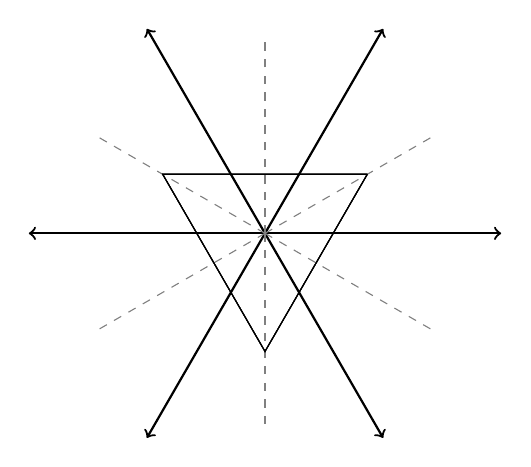
\begin{tikzpicture}[
    % arrow heads for all lines (with narrower arrow head width)
    %-{Straight Barb[bend,
       %width=\the\dimexpr10\pgflinewidth\relax,
       %length=\the\dimexpr12\pgflinewidth\relax]},
  ]
    %coordinate system
    %\draw[black] (-6,0) -- (6,0);
    %\draw[black] (0,-6) -- (0,6);
    % straight arrows
    \foreach \i in {0, 1, ..., 5} {
      \draw[->,thick, black] (0, 0) -- (\i*60:3);
    }
    \foreach \i in {0, 1, ..., 5} {
      \draw[dashed, gray] (0, 0) -- (30 + \i*60:2.5);
    }
    \foreach \i in {0, 2, 4 } {
      \draw[thin] (30:1.5 ) -- (150:1.5) -- (270:1.5) -- (30:1.5);
    }
  \end{tikzpicture}
  \hspace{1cm}
  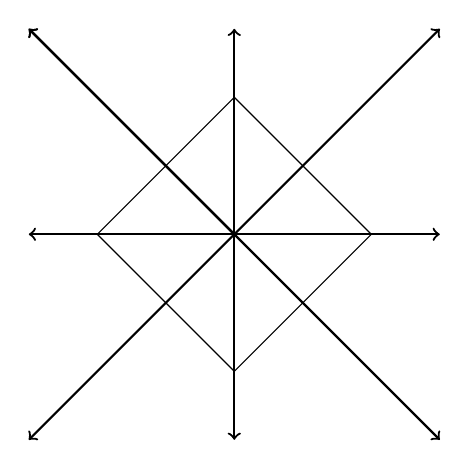
\begin{tikzpicture}[
    scale=0.87,
    % arrow heads for all lines (with narrower arrow head width)
    %-{Straight Barb[bend,
       %width=\the\dimexpr10\pgflinewidth\relax,
       %length=\the\dimexpr12\pgflinewidth\relax]},
  ]
    %coordinate system
    %\draw[black] (-6,0) -- (6,0);
    %\draw[black] (0,-6) -- (0,6);
    % straight arrows
    \foreach \i in {0, 1, ..., 3} {
      \draw[->,thick, black] (0, 0) -- (\i*90:3);
    }
    \draw[->,thick, black] (0, 0) -- (3,3);
    \draw[->,thick, black] (0, 0) -- (-3,3);
    \draw[->,thick, black] (0, 0) -- (-3,-3);
    \draw[->,thick, black] (0, 0) -- (-3,3);
    \draw[->,thick, black] (0, 0) -- (3,-3);
    \draw[thin] (2.0,0) -- (0,2.0) -- (-2.0,0) -- (0,-2.0) -- cycle;
  \end{tikzpicture}
  \caption{Die \weyl\hyp{}Gruppe des Wurzelsystems $\mathbf{A_2}$ (links) bildet die Symmetriegruppe $\mathbf{D_3}$ des eingezeichneten Dreiecks. Die gestrichelten Linien stellen die von den Wurzeln erzeugten Spiegelungsebenen dar. Im Falle des Wurzelsystems $\mathbf{B_2}$ (rechts) bildet die \weyl\hyp{}Gruppe die Symmetriegruppe $\mathbf{D_4}$ des Quadrats.}
\end{figure}

Es lassen sich nun unterschiedliche von $\W$ induzierte Gruppenoperationen betrachten. 
Ziel dieses Abschnittes ist es zu beweisen, dass die durch die Gruppe $\W$ auf der Menge der Fundamentalsysteme induzierte Gruppenoperation scharf transitiv ist.
Wir beginnen mit einer für beliebige Gruppenoperationen definierten Eigenschaft.

\begin{defn}
  Eine Gruppe $G$ operiere auf einer Menge $X$.
  Die Gruppenoperation $\circ \colon G \times X \to X$ heißt \emph{scharf transitiv}, wenn für alle $x,y \in X$ genau ein $g \in G$ existiert, sodass $g \circ x = y$ gilt. 
\end{defn}

Folgende Proposition gibt über die Wohldefiniertheit der von uns zu betrachtenden Gruppenoperationen Auskunft.

\begin{prop}
  \label{prop:groupOp}
  Sei $\Phi$ ein Wurzelsystem über $E$ mit \weyl\hyp{}Gruppe $\W$.
  Dann gelten für alle $\gamma, \gamma' \in E$ und $\sigma \in \W$ die folgenden Aussagen:
  \begin{enumerate}[(a)]
    \item Es operiert $\W$ auf der Menge der regulären Elemente: 
      \begin{addmargin}[2em]{2em}
        Es ist $\sigma(\gamma)$ genau dann regulär, wenn $\gamma$ regulär ist.
      \end{addmargin}
      
    \item Aus $\mathfrak{C}(\gamma) = \mathfrak{C}(\gamma')$ folgt, dass auch $\mathfrak{C}(\sigma(\gamma)) = \mathfrak{C}(\sigma(\gamma'))$. \\
      Es operiert $\W$ auf der Menge der \weyl\hyp{}Kammern $\{\mathfrak{C}(\omega) \mid \omega \text{ regulär}\}$. 
      Die Gruppenoperation lässt sich durch $ \sigma(\mathfrak{C}(\gamma)) = \mathfrak{C}(\sigma(\gamma))$ definieren.
      Das Bild einer \weyl\hyp{}Kammer ist also bereits durch das Bild eines Repräsentanten festgelegt.

    \item Es operiert $\W$ auf der Menge der Fundamentalsysteme $\{\Delta(\omega) \mid \omega \text{ regulär}\}$: 
      \begin{addmargin}[2em]{2em}
        Ist $\Delta$ ein Fundamentalsystem für $\Phi$, so auch $\sigma(\Delta)$. 
      \end{addmargin}

    \item Die unter (b) und (c) beschriebenen Gruppenoperationen sind kompatibel in dem Sinne, dass 
      $\sigma(\Delta(\gamma)) = \Delta(\sigma(\gamma))$
      und damit auch
      $\sigma(\mathfrak{C}(\Delta)) = \mathfrak{C}(\sigma(\Delta))$
      gilt.
  \end{enumerate}
\end{prop}

\begin{proof}
  (a): 
  Angenommen, $\sigma(\gamma)$ sei nicht regulär, dann existiert ein $\alpha \in \Phi$ mit $\sigma(\gamma) \in P_\alpha$.
  Damit folgt $\sigma(\gamma) = \sigma_\alpha \sigma(\gamma)$, da $\sigma_\alpha$ Elemente aus $P_\alpha$ fixiert.
  Hieraus ergibt sich mit Lemma \ref{lem:conjReflection} nun $\gamma = \sigma^{-1} \sigma_\alpha \sigma(\gamma) = \sigma_{\sigma(\alpha)}(\gamma)$, was wiederum $\gamma \in P_{\sigma(\alpha)}$ impliziert.
  Nach \hyperref[it:R3]{(R3)} gilt $\sigma(\alpha) \in \Phi$, also ist $\gamma$ im Widerspruch zur Voraussetzung nicht regulär.
  Die Annahme, dass $\sigma(\gamma)$ nicht regulär sei, muss also verworfen werden.
  
  Die Umkehrung der Aussage folgt aus der gezeigten Implikationsrichtung durch Anwendung der Spiegelung $\sigma^{-1}$ auf $\sigma(\gamma)$.

  (b): 
  Seien $\gamma, \gamma'$ regulär mit $\mathfrak{C}(\gamma) = \mathfrak{C}(\gamma')$.
  Angenommen, es sei $\mathfrak{C}(\sigma(\gamma)) \neq \mathfrak{C}(\sigma(\gamma'))$.
  Dann existiert ein $\alpha \in \Phi$, sodass einerseits $(\sigma(\gamma), \alpha) > 0$ und andererseits $(\sigma(\gamma'), \alpha) < 0$ gelten.
  Wir betrachten nun die Abbildung $x \mapsto  (\sigma(x), \alpha)$.
  Diese ist als Linearform auf dem endlichdimensionalen Vektorraum $E$ stetig bezüglich \euklid ischer Topologie.

  Da $\mathfrak{C}(\gamma)$ eine zusammenhängende Menge ist, folgt mit dem Zwischenwertsatz 
  %\cite[S.232]{bartsch2015allgemeine}
  , dass ein reguläres $x \in \mathfrak{C}(\gamma)$ existiert mit $(\sigma(x), \alpha) = 0$.
  Das bedeutet jedoch gerade, dass $\sigma(x)$ ein Element von $P_\alpha$ ist und damit wäre $\sigma(x)$ nicht regulär.
  Dies steht jedoch im Widerspruch zu (a). 
  Es muss also auch $\mathfrak{C}(\sigma(\gamma)) = \mathfrak{C}(\sigma(\gamma'))$ gelten.

  Also lässt sich die Gruppenoperation auf den \weyl\hyp{}Kammern repräsentantenunabhängig definieren und die Behauptung folgt.
  
  (c): 
  Da $\sigma$ als orthogonale Abbildung insbesondere injektiv ist, folgt, dass $\sigma(\Delta)$ wieder ein System linear unabhängiger Vektoren und damit aufgrund von \hyperref[it:B1]{(B1)} wieder eine Vektorraumbasis von $E$ ist.
  Zudem gilt $\sigma(\Delta) \subseteq \Phi$, da nach \hyperref[it:R3]{(R3)} diese Inklusion bereits für jeden Erzeuger $\sigma_\gamma$ von $\W$ mit $\gamma \in \Phi$ gilt.
  
  Ist nun $\beta \in \Phi$ mit der nach \hyperref[it:B2]{(B2)} existierenden Darstellung $\beta = \sum_{\alpha \in \Delta} k_\alpha \alpha$ gegeben, so gilt
  \begin{displaymath}
  \sigma(\beta) 
    = \sigma\Big(\,\sum_{\alpha \in \Delta} k_\alpha \alpha\Big)
    = \sum_{\alpha \in \Delta} k_\alpha \sigma(\alpha)
    = \sum_{\sigma(\alpha) \in \sigma(\Delta)} k_\alpha \sigma(\alpha)
  \end{displaymath}
  aufgrund der Linearität von $\sigma$.
  Die Vorzeichen der Linearfaktoren $k_\alpha$ bleiben zudem unverändert, womit \hyperref[it:B2]{(B2)} folgt.
  Damit ist auch $\sigma(\Delta)$ ein Fundamentalsystem.

  (d):
  Wir stellen zunächst fest, dass aufgrund der Aussage (c), die zu zeigende Gleichheit in dem Sinne wohldefiniert ist, dass $\sigma(\Delta(\gamma))$ als Bild eines Fundamentalsystems wieder ein Fundamentalsystem darstellt.

  Sei nun $\sigma(\alpha) \in \sigma(\Delta(\gamma))$.
  Mit $\alpha \in \Delta(\gamma)$ gilt definitionsgemäß $(\alpha, \gamma) > 0$.
  Spiegelungen erhalten als Isometrien das Skalarprodukt, es gilt also auch $(\sigma(\alpha), \sigma(\gamma)) > 0$.
  Dies wiederum impliziert $\sigma(\alpha) \in \Phi^+(\sigma(\gamma))$.
  Angenommen, $\sigma(\alpha)$ wäre eine zerlegbare Wurzel.
  Dann ist auch $\alpha$ zerlegbar, da $\sigma$ bijektiv ist.
  Dies steht jedoch im Widerspruch dazu, dass mit $\alpha \in \Delta$ die Wurzel $\alpha$ als einfach vorausgesetzt wurde.
  Also muss $\sigma(\alpha)$ auch einfach sein, womit $\sigma(\alpha) \in \Delta(\sigma(\gamma))$ folgt.
  Das impliziert die Gültigkeit der Inklusion $\sigma(\Delta(\gamma)) \subseteq \Delta(\sigma(\gamma))$.
  
  Da $\sigma$ bijektiv ist und beide Mengen als Teilmengen des endlichen Wurzelsystems $\Phi$ auch endlich sind, folgt hiermit bereits die Gleichheit.
\end{proof}

Nun zu dem zentralen Satz dieser Ausarbeitung.

\begin{samepage}
\begin{thm}
  \label{thm:simplyTransitive}
  Es sei $\Delta$ ein Fundamentalsystem des Wurzelsystems $\Phi$ über $E$ mit zugehöriger \weyl\hyp{}Gruppe $\W$.
  Dann gelten die folgenden Aussagen:
  \begin{enumerate}[(a)]

    \item Wenn $\gamma \in E$ regulär ist, dann existiert ein $\sigma \in \W$, sodass für alle $\alpha \in \Delta$ die Ungleichung $(\sigma(\gamma), \alpha) > 0$ gilt. 
      Es operiert $\W$ also transitiv auf der Menge der \weyl\hyp{}Kammern.

    \item Wenn $\Delta'$ ein weiteres Fundamentalsystem von $\Phi$ ist, dann existiert ein $\sigma \in \W$, sodass $\sigma(\Delta') = \Delta$ gilt.
      Es operiert $\W$ also transitiv auf der Menge der Fundamental\-systeme.

    \item Für alle $\alpha \in \Phi$ existiert ein $\sigma \in \W$ mit $\sigma(\alpha) \in \Delta$.
      Jede Wurzel liegt also in der $\W$\hyp{}Bahn einer einfachen Wurzel.

    \item Die \weyl\hyp{}Gruppe $\W$ wird erzeugt von den Spiegelungen $\sigma_\alpha$ für $\alpha \in \Delta$.

    \item Ist $\sigma \in \W$ und gilt $\sigma(\Delta) = \Delta$, so folgt $\sigma = \mathds{1}$.
      Also operiert $\W$ scharf transitiv auf der Menge der Fundamental\-systeme.
  \end{enumerate}
\end{thm}
\end{samepage}

\begin{proof}
  Wir führen die Beweise für (a) bis (c) zunächst für die von den einfachen Spiegelungen erzeugte Untergruppe $\W'$ von $\W$ und beweisen damit auf den ersten Blick stärkere Aussagen.
  Nach dem Beweis von (d) folgt $\W' = \W$.

  (a):
  Es sei $\gamma \in E$ regulär und $\delta := \tfrac{1}{2} \sum_{\alpha \in \Phi^+} \alpha$.
  Da nach Lemma \ref{lem:weylFinite} die \weyl\hyp{}Gruppe und damit auch die Untergruppe $\W'$ endlich sind, existiert ein $\sigma \in \W'$, sodass $(\sigma(\gamma), \delta)$ maximal wird.
  Für alle $\alpha \in \Delta$ gilt $\sigma_\alpha\sigma \in \W'$ aufgrund der Untergruppeneigenschaft.
  Daraus folgt
  \begin{align*}
    (\sigma(\gamma), \delta) 
    &\geq (\sigma_\alpha \sigma(\gamma), \delta) &&\text{aufgrund der Maximalitätseigenschaft von $(\sigma(\gamma),\delta)$} \\
    &= (\sigma(\gamma), \sigma_\alpha(\delta)) &&\text{da $\sigma_\alpha$ eine Isometrie und zudem selbstinvers ist} \\
    &= (\sigma(\gamma), \delta - \alpha) &&\text{nach Korollar \ref{cor:sigmaDelta}} \\
    &= (\sigma(\gamma), \delta) - (\sigma(\gamma), \alpha) &&\text{aufgrund der Bilinearität des Skalarproduktes.}
  \end{align*}
  Also muss $(\sigma(\gamma), \alpha) \geq 0$ für alle $\alpha \in \Delta$ gelten, um nicht der Maximalität von $\sigma$ zu widersprechen.

  Nach Voraussetzung ist $\gamma$ regulär.
  Daher kann für kein $\alpha \in \Delta$ die Identität $(\sigma(\gamma),\alpha) = 0$ gelten, da sonst $\gamma$ in $P_{\sigma^{-1}(\alpha)}$ liegt, was der vorausgesetzten Regularität widerspricht.
  Somit gilt für alle $\alpha \in \Delta$ die strikte Ungleichung $(\sigma(\gamma), \alpha) > 0$.
  Das bedeutet jedoch gerade, dass $\sigma(\gamma)$ in der Fundamentalkammer $\mathfrak{C}(\Delta)$ liegt.

  Also bildet die einfache Spiegelung $\sigma$ entsprechend Proposition \ref{prop:groupOp} die \weyl\hyp{}Kammer $\mathfrak{C}(\gamma)$ auf $\mathfrak{C}(\Delta)$ ab. 
  Somit gilt, dass alle \weyl\hyp{}Kammern mit der Fundamentalkammer verbunden sind
  Die Menge der \weyl\hyp{}Kammern ist also eine $\W'$\hyp{}Bahn und die Gruppenoperation damit transitiv.

  (b):
  Nach Satz \ref{thm:base} korrespondieren Fundamentalsysteme zu regulären Elementen.
  Sind also $\gamma, \gamma'$ reguläre Elemente und $\Delta(\gamma)$, $\Delta(\gamma')$ zwei Fundamentalsysteme, so entsprechen diesen nach Lemma \ref{lem:correspondenceOfChambers} in eindeutiger Weise auch \weyl\hyp{}Kammern $\mathfrak{C}(\gamma), \mathfrak{C}(\gamma')$.
  Da nach dem vorangehenden Beweis die Untergruppe $\W'$ die \weyl\hyp{}Kammern transitiv permutiert, gilt dies auch für die korrespondierende Gruppenoperation auf Fundamentalsystemen aus Proposition \ref{prop:groupOp}.
  
  (c):
  Da nach (b) die Untergruppe $\W'$ transitiv auf der Menge der Fundamentalsysteme operiert, genügt es nachzuweisen, dass jede Wurzel $\alpha \in \Phi$ in einem Fundamentalsystem enthalten ist.
  Aufgrund von Axiom \hyperref[it:R2]{(R2)} sind $\pm \alpha$ die einzigen zu $\alpha$ proportionalen Wurzeln in $\Phi$.
  Somit unterscheiden sich alle Hyperebenen $P_\beta$ von $P_\alpha = P_{-\alpha}$.
  Nach Proposition \ref{prop:unterraumAusschoepfung} lässt sich $P_\alpha$ nicht von den echten Unterräumen $P_\alpha \cap P_\beta$ mit $\alpha \neq \beta$ ausschöpfen.
  Es existiert daher ein $\gamma \in P_\alpha$ mit $\gamma \not\in P_\beta$ für alle $\beta \neq \pm\alpha$.

  Entsprechend Satz \ref{thm:base} korrespondiert zu jedem regulären Element ein Fundamentalsystem. 
  Es gilt nun in der Nähe von $\gamma$ ein geeignetes reguläres Element zu finden und nachzuweisen, dass $\alpha$ in dem entsprechenden Fundamentalsystem enthalten ist.

  Wir wählen dazu ein $\varepsilon > 0$ und $\gamma' \in E$ möglichst nahe bei $\gamma$, sodass $(\gamma', \alpha) = \varepsilon > 0$ ist und $|(\gamma', \beta)| > \varepsilon$ für alle $\beta \neq \pm \alpha$ gilt ($\ast$).
  Dies ist möglich, da nach Konstruktion $(\gamma, \beta) \neq 0$ für alle $\beta \neq \pm \alpha$ gilt.
  Damit existiert aufgrund der Stetigkeit des Skalarproduktes und der Betragsfunktion ein $\delta > 0$, sodass für alle $\gamma' \in B_\delta(\gamma)$ auch $\varepsilon < |(\gamma', \beta)|$ gilt, falls man $\varepsilon = \tfrac{1}{2} \min_{\beta \neq \pm\alpha}{|(\gamma,\beta)|}$ wählt.
  Das Komplement der Hyperebene $P_\alpha$ liegt dicht in $E$ und folglich besitzt $P_\alpha$ keine inneren Punkte.
  Also existiert ein $\gamma' \in B_\delta(\gamma) \setminus P_\alpha$ und wir können durch Verkleinerung von $\varepsilon$ und eventuelle Multiplikation von $\gamma'$ mit $-1$ annehmen, dass $(\gamma', \alpha) = \varepsilon$ gilt, weil $B_\delta(\gamma)$ zusammenhängend ist.

  Nach Konstruktion ist $\gamma'$ regulär.
  Zudem ist $\alpha$ bezüglich $\Phi^+(\gamma')$ unzerlegbar.
  Denn wäre $\alpha$ zerlegbar, so existieren $\beta_1, \beta_2 \in \Phi^+(\gamma')$ mit $\alpha = \beta_1 + \beta_2$.
  Mit der Bilinearität des Skalarproduktes folgt dann jedoch unter Berücksichtigung von ($\ast$)
  \begin{displaymath}
    \varepsilon 
    = (\gamma', \alpha) 
    = (\gamma', \beta_1 + \beta_2) 
    = (\gamma', \beta_1) + (\gamma', \beta_2)
    = |(\gamma', \beta_1)| + |(\gamma', \beta_2)|
    > \varepsilon + \varepsilon
    = 2\varepsilon,
  \end{displaymath}
  also ein Widerspruch.
  Folglich ist $\alpha$ unzerlegbar bezüglich $\Phi^+(\gamma')$, was $\alpha \in \Delta(\gamma')$ impliziert.

  (d):
  Da nach Konstruktion $\W'$ eine Untergruppe von $\W$ ist, reicht es zu zeigen, dass jede Spiegelung $\sigma_\alpha$ mit $\alpha \in \Phi$ ein Element von $\W'$ ist.
  Nach (c) existiert ein $\sigma \in \W'$, sodass $\beta := \sigma(\alpha) \in \Delta$.
  Damit gilt insbesondere $\sigma_\beta \in \W'$.
  Aufgrund von Lemma \ref{lem:conjReflection} ist $\sigma_\beta = \sigma_{\sigma(\alpha)} = \sigma \sigma_\alpha \sigma^{-1}$, also folgt mit der Untergruppeneigenschaft von $\W'$ sodann $\sigma_\alpha = \sigma^{-1} \sigma_\beta \sigma \in \W'$.
  Folglich gilt $\W' = \W$ und alle bereits für $\W'$ bewiesenen Aussagen gelten auch für $\W$.

  (e):
  Sei $\sigma \in \W$ mit $\sigma(\Delta) = \Delta$.
  Nehmen wir $\sigma \neq \mathds{1}$ an, so lässt sich nach (d) die Abbildung $\sigma$ als Produkt $\sigma = \sigma_{\alpha_1}\dots\sigma_{\alpha_t}$ schreiben, wobei $\alpha_1,\dots,\alpha_t$ einfache Wurzeln seien. 
  Nach der konstruktiven Definition des Hüllenoperators für Gruppen können wir zusätzlich annehmen, dass $t$ minimal gewählt sei.
  Dann ist nach Korollar \ref{cor:minimalReflection} das Bild $\sigma(\alpha_t)$ negativ, also gilt insbesondere $\sigma(\alpha_t) \not\in \Delta$ im Widerspruch zur Voraussetzung.
  Die Annahme muss also verworfen werden und es folgt $\sigma = \mathds{1}$.

  Es soll nun gezeigt werden, dass hieraus bereits die scharfe Transitivität der Gruppenoperation folgt.
  Dazu seien $\Delta_1,\Delta_2$ Fundamentalsysteme und $\sigma \in \mathcal{W}$ die nach (b) existierende Abbildung mit $\sigma(\Delta_1) = \Delta_2$.
  Ist $\sigma'$ eine weitere Abbildung mit $\sigma'(\Delta_1) = \Delta_2$, so gilt insbesondere $\sigma^{-1} \sigma'(\Delta_1) = \sigma^{-1}(\Delta_2) = \sigma(\Delta_2) = \Delta_1$.
  Nach (c) existiert zudem ein $\mu \in \W$ mit $\mu(\Delta) = \Delta_1$.
  Damit folgt $\sigma^{-1} \sigma' \mu (\Delta) = \mu (\Delta)$ oder äquivalent $\mu^{-1} \sigma^{-1} \sigma' \mu (\Delta)$.
  Mit dem vorangehenden Absatz folgt sogleich $\mu^{-1} \sigma^{-1} \sigma' \mu = \mathds{1}$ und daraus $\sigma = \sigma'$.
  Also operiert $W$ sogar scharf transitiv auf der Menge der Fundamentalsysteme.
\end{proof}

Aus der Tatsache, dass $\W$ von einfachen Spiegelungen erzeugt wird, lassen sich nun weitere Aussagen folgern.

\begin{defn}
  Sei $\Phi$ ein Wurzelsystem mit Fundamentalsystem $\Delta$ und \weyl\hyp{}Gruppe $\W$. 
  Des Weiteren sei $\sigma \in \W$, mit einer Darstellung $\sigma = \sigma_{\alpha_1}\dots\sigma_{\alpha_t}$ ($\ast$), wobei $t$ minimal gewählt sei und $\alpha_i \in \Delta$ gelte. 
  Dann nennt man den Ausdruck ($\ast$) auch \emph{reduziert} und definiert die \emph{Länge von $\sigma$ bezüglich} $\Delta$ durch $\ell(\sigma) := t$.
\end{defn}

\begin{lem}
  \label{lem:lengthAndNegativeRoots}
  Sei $\Phi$ ein Wurzelsystem über $E$ mit Fundamentalsystem $\Delta$ und $\W$ die zugehörige \weyl\hyp{}Gruppe.
  Für $\sigma \in \W$ bezeichne $n(\sigma)$ die Anzahl der positiven Wurzeln $\alpha$ mit negativem Bild $\sigma(\alpha)$.
  Dann gelten die folgenden Aussagen:
  \begin{enumerate}[(1)]
    \item Sei $\alpha \in \Delta$. Falls $\sigma(\alpha)$ negativ ist, so gilt $n(\sigma\sigma_\alpha(\alpha)) = n(\sigma) - 1$.
    \item Es gilt $\ell(\sigma) = n(\sigma)$.
  \end{enumerate}
\end{lem}

\begin{proof}
  (1):
  Sei $\sigma(\alpha)$ negativ.
  Aus Lemma \ref{lem:permute} folgt, dass $\sigma_\alpha$ alle von $\alpha$ verschiedenen positiven Wurzeln permutiert.
  Einerseits enthält $\sigma(\Phi^+ \setminus \{\alpha\})$ somit genauso viele negative Wurzeln wie $\sigma(\sigma_\alpha(\Phi^+ \setminus \{\alpha\}))$.
  Andererseits ist jedoch 
  $\sigma \sigma_\alpha (\alpha) = \sigma(-\alpha) = -\sigma(\alpha)$ 
  positiv.
  Daraus können wir $n(\sigma\sigma_\alpha) = n(\sigma) - 1$ folgern.

  (2):
  Wir führen den Beweis mittels Induktion über $\ell(\sigma)$.

  Ist $\ell(\sigma)=0$, so gilt $\sigma = \mathds{1}$, was wiederum $n(\sigma)=0$ zur Folge hat.

  Angenommen, die Behauptung gelte für alle $\tau \in \W$ mit $\ell(\tau) < \ell(\sigma)$.
  Wir schreiben nun $\sigma$ als reduzierten Ausdruck $\sigma = \sigma_{\alpha_1} \dots \sigma_{\alpha_t}$ und definieren $\alpha := \alpha_t$.
  Über Korollar \ref{cor:minimalReflection} folgt damit die Negativität von $\sigma(\alpha)$.
  Aufgrund von (1) können wir einerseits $n(\sigma\sigma_\alpha) = n(\sigma) - 1$ folgern.
  Andererseits gilt 
  \begin{displaymath}
  \ell(\sigma\sigma_\alpha) 
  = \ell(\sigma_{\alpha_1} \dots \sigma_{\alpha_{t}} \sigma_{\alpha_t}) 
  = \ell(\sigma_{\alpha_1} \dots \sigma_{\alpha_{t -1}}) 
  = \ell(\sigma) - 1 < \ell(\sigma).
  \end{displaymath}
  Mit der Induktions\-voraussetzung folgt somit $\ell(\sigma\sigma_\alpha) = n(\sigma\sigma_\alpha)$, also $\ell(\sigma) - 1 = n(\sigma) - 1$, woraus sich die Behauptung ergibt.
\end{proof}

Nun betrachten wir die einfach transitive Operation der \weyl\hyp{}Gruppe auf den \weyl\hyp{}Kammern aus Satz \ref{thm:simplyTransitive}.
Es soll gezeigt werden, dass der in der \euklid ischen Topologie gebildete Abschluss $\overline{\mathfrak{C}(\Delta)}$ der Fundamentalkammer bezüglich des Fundamentalsystems $\Delta$ ein \emph{Fundamentalbereich} der natürlichen Gruppenoperation von $\W$ auf $E$ ist.
Dies bedeutet, dass für alle Vektoren $x \in E$ genau ein $y \in \overline{\mathfrak{C}(\Delta)}$ existiert mit $x \in \W y = \{\sigma(y) \mid \sigma \in \W\}$.

\begin{lem}
  \label{lem:fundamentalDomain}
  Sei $\Phi$ ein Wurzelsystem über $E$ mit Fundamentalsystem $\Delta$ und $\W$ die zugehörige \weyl\hyp{}Gruppe.
  Dann gelten folgende Aussagen:
  \begin{enumerate}[(1)]
    \item Jeder Punkt aus $E$ liegt in der $\W$\hyp{}Bahn eines Elementes aus  $\overline{\mathfrak{C}(\Delta)}$.
    \item Falls für $\lambda, \mu \in \overline{\mathfrak{C}(\Delta)}$ ein $\sigma \in \W$ existiert mit $\sigma (\lambda) = \mu$, dann ist $\sigma$ das Produkt einfacher Spiegelungen, die $\lambda$ fixieren, und es gilt $\lambda = \mu$.
  \end{enumerate}
  Insbesondere ist $\overline{\mathfrak{C}(\Delta)}$ ein Fundamentalbereich der natürlichen Gruppenoperation der Gruppe $\W$ auf dem Vektorraum $E$.
\end{lem}

Eine Verschärfung von Lemma \ref{lem:fundamentalDomain} findet sich in \cite[S.22]{humphreys1992reflection}.

\begin{proof}
  (1):
  Wir setzen die in Abschnitt \ref{sec:grundlagen} auf der Menge der Wurzeln $\Phi$ definierte Halb\-ordnungsrelation $\succeq$ nun auf ganz $E$ fort, indem wir genau dann $\beta \preceq \alpha$ setzen, wenn $\alpha - \beta$ eine $\R$-Linearkombination mit sämtlich positiven Koeffizienten ist oder $\alpha = \beta$ gilt.

  Sei $\lambda \in E$ gegeben. 
  Wir betrachten als nächstes die Teilmenge $M$ aller $\W$\hyp{}Bahnelemente $\mu \in \W\lambda$, für die $\mu \succeq \lambda$ gilt.
  Da $M$ nach Lemma \ref{lem:weylFinite} endlich und aufgrund von $\lambda \in M$ nichtleer ist, existieren bezüglich der Halbordnung $\succeq$ maximale Elemente.

  Sei $\mu = \sigma(\lambda)$ mit $\sigma \in \W$ ein solches maximales Element.
  Wir möchten nun zeigen, dass $\mu \in \overline{\mathfrak{C}(\Delta)}$ gilt.
  Sei dazu $\alpha \in \Delta$.
  Es ist $\sigma_\alpha(\mu) = \mu - \langle \mu, \alpha \rangle \alpha$.
  Da $\sigma_\alpha(\mu) = \sigma_\alpha \sigma (\lambda) \in \W\lambda$ gilt, folgt $\langle \mu, \alpha \rangle \geq 0$ beziehungsweise $(\mu,\alpha) \geq 0$, um nicht der Maximalität von $\mu$ zu widersprechen.
  Da $\alpha$ beliebig war, liegt somit $\mu$ in $\overline{\mathfrak{C}(\Delta)}$.

  (2):
  Wir führen einen Induktionsbeweis über die Länge $\ell(\sigma)$.
  Nach der konstruktiven Definition des Hüllenoperators für Gruppen und Satz \ref{thm:simplyTransitive} lässt sich annehmen, dass $\sigma_\alpha$ bereits Produkt einfacher Spiegelungen ist.

  Ist $\ell(\sigma) = 0$, so folgt $\sigma = \mathds{1}$, womit sich $\lambda = \mathds{1}(\lambda) = \sigma(\lambda) = \mu$ ergibt.

  Sei nun $\ell(\sigma) > 0$ und die Aussage für alle $\tau \in \W$ mit $\ell(\tau) < \ell(\sigma)$ bereits bewiesen.
  Nach Lemma \ref{lem:lengthAndNegativeRoots} bildet $\sigma$ eine positive Wurzel auf eine negative Wurzel ab.
  
  Insbesondere existiert also eine einfache Wurzel $\alpha \in \Delta$ mit negativem Bild $\sigma(\alpha)$.
  Für alle $\xi \in \mathfrak{C}(\Delta)$ gilt $(\xi, \sigma(\alpha)) = \sum_{\beta \in \Delta} k_\beta (\xi,\beta) < 0$, denn alle $k_\beta$ sind nach Voraussetzung negativ und gilt $(\xi,\beta) > 0$, weil $\xi$ als Element der Fundamentalkammer mit allen einfachen Wurzeln einen spitzen Winkel einschließt.
  Da $\mu \in \overline{\mathfrak{C}(\Delta)}$ vorausgesetzt wurde existiert eine Folge $(\xi_n)_{n \in \N}$ in $\mathfrak{C}(\Delta)$ mit $\lim_{n \to \infty} \xi_n = \mu$.
  Aufgrund der Stetigkeit des Skalarproduktes ergibt sich somit einerseits
  \begin{displaymath}
    (\lambda,\alpha)
    = (\sigma(\mu),\alpha)
    = (\mu, \sigma(\alpha)) 
    = (\lim_{n \to \infty} \xi_n, \sigma(\alpha)) 
    = \lim_{n \to \infty} ( \xi_n, \sigma(\alpha)) \leq 0,
  \end{displaymath}
  weil $\sigma$ eine Isometrie ist.
  Andererseits folgt aus $\lambda \in \overline{\mathfrak{C}(\Delta)}$ auch $0 \leq (\lambda,\alpha)$, da $\lambda = \lim_{n \to \infty} \eta_n$ für $\eta_n \in \mathfrak{C}(\Delta)$.

  Hieraus folgt $(\lambda, \alpha) = 0$, also gilt $\lambda \in P_\alpha$.
  Dies wiederum impliziert $\sigma_\alpha(\lambda) = \lambda$ und weiter noch $\sigma \sigma_\alpha(\lambda) = \mu$.
  Somit erfüllt $\sigma \sigma_\alpha$ die Voraussetzungen des zu beweisenden Lemmas. 

  Wir zeigen nun, dass auf $\sigma \sigma_\alpha$ auch die Induktionsannahme zutrifft.
  Nach Lemma \ref{lem:lengthAndNegativeRoots}(1) gilt $n(\sigma\sigma_\alpha) = n(\sigma) - 1$, woraus schließlich mit \ref{lem:lengthAndNegativeRoots}(2) die Gleichheit $\ell(\sigma\sigma_\alpha) = \ell(\sigma) - 1$ folgt.
  Es gilt also $\ell(\sigma\sigma_\alpha) < \ell(\sigma)$ und darum lässt sich aufgrund der Induktionsannahme $\lambda = \mu$ folgern.
\end{proof}

